% $Id: introduction.tex 65669 2015-01-09 14:55:20Z tgershon $

\section{Investigation of $\Bd \rightarrow \Kstar(892) \etaz$}
\label{sec:Analysis}
%motivation and stuff here TODO


The intention of this analysis is to use the full $3fb^{-1}$ dataset collected by \lhcb in run I of the LHC.  However, the $1fb^{-1}$ of data collected at a 7TeV centre of mass energy (CoM) and the $2fb^{-1}$ of data collected at an 8TeV centre of mass energy will be treated seperatley at least for the selection stage of this analysis.  This is because the differences in kinematic variables between these two CoM energies would make a common selection for both sub-optimal. So far only the $2fb^{-1}$ of 8TeV data has been considered, therefore all results in this report are based on that dataset.

\subsection{Decay Reconstruction}
\label{sec:Decay Reconstruction}
The \Kstar will be reconstructed in the channel $\Kstar \to \Kp\pim$ which has a branching fraction of $99.901\pm0.009\%$ \cite{PDG2014}.  The \etaz will be reconstructed in the channel $\etaz \to \pip\pim\piz$ where the \piz decays to 2 photons, which has a combined branching fraction of $21.83\pm0.28\%$\cite{PDG2014}.  This is not the dominant decay mode of the \etaz particle but the 2 decay modes with higher branching fractions contain only neutral particles in the final state.  This means there is no tracking information available and the \lhcb calorimeter (unlike the \atlas calorimeter) does not provide any directional information for the photons it detects.  Consequently, reconstruction efficiencies for all neutral final states are significantly lower and backgrounds are higher, which makes the \pip\pim\piz channel the optimal choice.  

Each of the final state particles in the decay chain are assigned a mass hypothesis based on information from all of the \lhcb sub detectors before being combined to form their respective mother particles.  The properties of the mother particle (e.g Energy, momentum, flight distance) are then determined with a fit to the daughter particles;   the $\chi^2$ of this fit can then aid the choice of candidate decays.

The combination of particles to form a \Bd candidate described is all done by the \lhcb reconstruction packages and the initial, loose, selection of \Bd candidates is based on this reconstruction. However, a better mass resolution can be achieved by refitting the entire decay tree of \Bd candidates whilst applying extra constraints.  This technique was first used by the \babar and is practically implemented with a Kalman fitter\cite{Hulsbergen:2005pu}.  Most commonly, any intermediate daughter particles are constrained to have their known masses and all tracks are constrained to come from the position where the hard pp interaction took place (primary vertex).  In this analysis all daughter particles are constrained to come from the primary vertex and the \etaz mass is constrained to the current world average ($547.826\pm0.018MeV$)\cite{PDG2014}.  The \Kstar mass is not constrained because it is a wide resonance; the natrual width of the \Kstar is around 50MeV.  It is impossible to reconstruct a particle with a better resolution than what is dictated by it's natural width.  Consequently,, one can expect correctly reconstructed \Kstar particles to still have a mass a considerable distance from the PDG value.  Therefore, constraining the \Kstar candidate to its PDG value can bias the refitted \Bd mass.

\subsection{Event Selection}
\label{sec:Selection}

The first stage of any analysis is selecting a subset of the \lhcb dataset that contains a high purity of events of interest to the analysis.  Essentially, one has to mimise the number of background events that pass a set of selection criteria whilst keeping as many signal events as possible. These selection criteria are composed of several stages.

\subsubsection{Stripping Selection}
\label{sec:Stripping}
As the data collected by \lhcb in run I is of the order of 10s of Petabytes it is impossible for every user to start with the full dataset.  Therefore, loose selection criteria need to be applied to the full dataset to produce a subset of data that can be worked with.  A set of these loose selection criteria are refered to as a stripping line, some of which are quite general (e.g dimuon final state) whereas others are for a specific analysis.  The amount of CPU time taken to run over the full run I dataset is very large, therefore stripping takes place when the data is taken and then incremental re-strippings take place no more than a few times a year.  The stripping process is always run centrally.
%TODO check how to make a stripping line
The cuts that go into a stripping line are determined such that they give maximal signal efficiency whilst keeping within the amount of per event CPU time allocated to that stripping line.  The signal efficiencies are assessed by applying the same selection to simulated (MC) signal events.  In the case of this analysis, the stripping line was already completed before this analysis started otherwise the deadline for submitting stripping lines would not have been met.

The cuts applied as part of the stripping selection used for this analysis are shown in Table \ref{tab:stripping}.

\begin{table}[h]
  \label{tab:stripping}
  \scriptsize
  \centering
  \begin{tabular}{ccc}
    \hline
    Particle      & Cut            & Value      \\ \hline
    \Bz          & \chisqvtx$<$   & 15         \\
    & DOCA \chisq$<$ & 20           \\
    & \pt $>$        & 1500\mev     \\
    & DIRA $>$       & 0.9995       \\
    & IP \chisq $<$  & 20           \\
    & m(\Bz)$\pm$    & 750\mev      \\ \hline
    \Peta & \chisqvtx$<$   & 15           \\
    & DOCA \chisq$<$ & 20           \\
    & \pt $>$        & 2000\mev     \\
    & m(\etaz)$\pm$ & 100\mev \\ \hline
    Track        & \pt $>$        & 300\mev      \\
    & Ghost Prob $<$ & 0.5          \\\hline
    \Kstar     & \chisqvtx$<$     & 9        \\
    & IP \chisq$<$     & 5        \\
    & \pt $>$          & 1200\mev \\
    & m(\Kstar)$\pm$   & 100MeV   \\ 
    & Daughter \pt $>$ & 500\mev  \\\hline
  \end{tabular}
  \caption{The stripping selection applied}
\end{table}

The meaning of these variables is as follows:
\begin{itemize}
\item \textbf{$\chi_{vtx}^2$} is the $\chi^2$ per degree of freedom of the initial vertex fit used to determine the properties of the daughter particles (see section \label{sec:Decay Reconstruction}).
\item \textbf{DOCA $\chi^2$} requires the $\chi^2$ of the distance of closest approach between all possible pairs of particles that form the \Bd to be less than the given value
\item \textbf{$P_t$} Momentum transverse to the beam pipe.
\item \textbf{DIRA} The cosine of the angle between the \Bd momentum direction and the vector between the most likely primary vertex and the \Bd decay vertex.
\item \textbf{IP $\chi^2$} The $\chi^2$ of the impact parameter (see Figure \ref{fig:decaydiag}).
\item \textbf{m(X)$\pm$} Requires the mass of the candidate to lie no more than this value from the PDG mass.
\item \textbf{Ghost Prob} The probability that a track is fake, as determined by the \lhcb tracking system.
\end{itemize}
In addition to the cuts shown in Table \ref{tab:stripping}, candidates are required to pass either of the  ``HLT1TrackAllL0Decision'' trigger lines which are explained in section \ref{sec:trigger}.


The efficiency of this selction can be assessed by applying it to signal MC; the efficiency is then simply $\frac{No. True Signal Events Passing Stripping}{ No. Generated}$.  The stripping efficiency is found to be $0.00317 \pm 0.00002$, which is a quite typical stripping efficiency at \lhcb.
%However, when the \lhcb analysis software is ran on MC not every resulting event is a true signal event.  This is because false candidates can easily be created for a variety of reasons, but the most common of which is when particles from other pp interactions in the same bunch crossing get wrongly attributed as a candidate particle.  To ensure only true MC signal events are used in this analysis truth cuts are applied before it is used.

The stripping efficiency is then found to be $0.00317 \pm 0.00002$, which is a quite typical stripping efficiency at \lhcb.

\subsubsection{Trigger}
\label{sec:trigger}
\lhcb has many trigger selections (trigger lines) that are applied as part of the triggering process, each of which is tailored towards a set of analyses with common properties. If an event passes any of these trigger lines it is stored, but the specific trigger lines that it passed are flagged.  Therefore, the next step of the analyses is to require events to pass trigger lines more specific to this analysis.

When an event passes a trigger line it can be described as triggered on signal (TOS) or triggered independent of signal (TIS).  TOS is when a candidate signal particle, or any component of the event contributing to it's reconstruction, causes the event to pass the trigger line.  More specifically, a minimum of $70\%$ of the trigger objects (e.g track, calorimeter cluster) that caused the event to pass the trigger line have to belong to the signal candidate. An event is classified as TIS if objects not used to reconstruct the signal candidate caused the caused the event to pass the trigger line \cite{1748-0221-8-04-P04022}. This TIS and TOS information can be used to perform a data driven assessment of triggering efficiencies, although this is not performed for this analysis(yet)\cite{Tolk:1701134}.

In order to pass the trigger selection, an event must satisfy the following criteria:
\textit{
  (L0GlobalTIS \textbf{OR} L0HadronDecision TOS) \textbf{AND} (Hlt1TrackAllL0Decision TOS) \textbf{AND} (Hlt2Top2BodyBBDTDecision TOS \textbf{OR} B0 Hlt2Topo3BodyBBDTDecision TOS \textbf{OR} Hlt2Topo4BodyBBDTDecision TOS)
}

The L0 Hadron Decision TOS line is required because the final state of this analysis contains 4 hadrons, therefore events that do not pass this trigger line are unlikely to be signal.  The Hlt2 trigger lines make use of the fact that this stage of the trigger is applied offline and apply a boosted decision tree (BDT) using topological variables, more description of BDTs is given in section \ref{sec:multivar}.

As part of the monte carlo production process the \lhcb trigger system is emulated, therefore MC events are also flagged with the trigger lines they pass.  This means the signal efficiecny of this trigger selection can be assessed simply by applying it to MC.  The signal efficiency of this trigger selection is found to be $0.715\pm0.006$.  This is a good trigger efficiency for \lhcb, and considerably higher than the approximately $20\%$ efficiency that hampered the analysis of \Lb \to \Lz\etaz \cite{LHCb-PAPER-2015-019}.

\subsubsection{Multivariate Selection}
\label{sec:multivar}
There are many kinematic and detector variables associated with every event that can be used to discriminate signal events from background events.  However, applying cuts to these variables individually does not provide optimal signal and background seperation.  Furthermore, there are often correlations between the variables that are difficult to account for when individual cuts are used.  For both of these reasons a multivariate selection procedure is applied in this analysis which makes use of all the available variables at the same time.  It has been seen in many other \lhcb analyses that the most effective type of multivariate analysis is a boosted decision tree(BDT).  BDT's were first developed as a way of perforiming particle identification at the MiniBooNE neutrino experiment but have since been used very widely within HEP experiments as well \cite{2005NIMPA.555..370Y}.

\paragraph{Decision Tree}
A simple decision tree (DT) is just a set of binary cuts applied one after the other to decide if an event is signal or background.  Each cut is known as a node. The positions of these cuts are chosen (trained) based on control samples of data that are known to be signal and background.  The gini index is given by, $G=P(1-P)$ where P is the purity of a subset of events.  At each node the positon of the cut is chosen to optimise the criterion C which is given by,

\begin{equation}
  C=G_{node}-G_{passing}-G_{not passing}
\end{equation}

An example of a trained DT is shown in Figure \ref{fig:DT}.  Every event in this tree has the initial selection criteria at the top of the tree applied, and then the further cuts are applied depending on the output of the first.  Every event is then classified as signal or background by this tree.

The specific tree shown in Figure \ref{fig:DT} has been used to classify artificial events just based on the variables $x$ and $y$.  Figure \ref{fig:square} shows a scatter plot of $x$ against $y$ populated by both ``signal'' and ``background'' events.  The positions of the cuts applied by this DT are also shown; it can be seen they seperate signal and background reasonably well.  If more variables are used, more nodes can be added to the decision tree and the cuts become multi dimensonial.
\begin{figure}
  \centering
  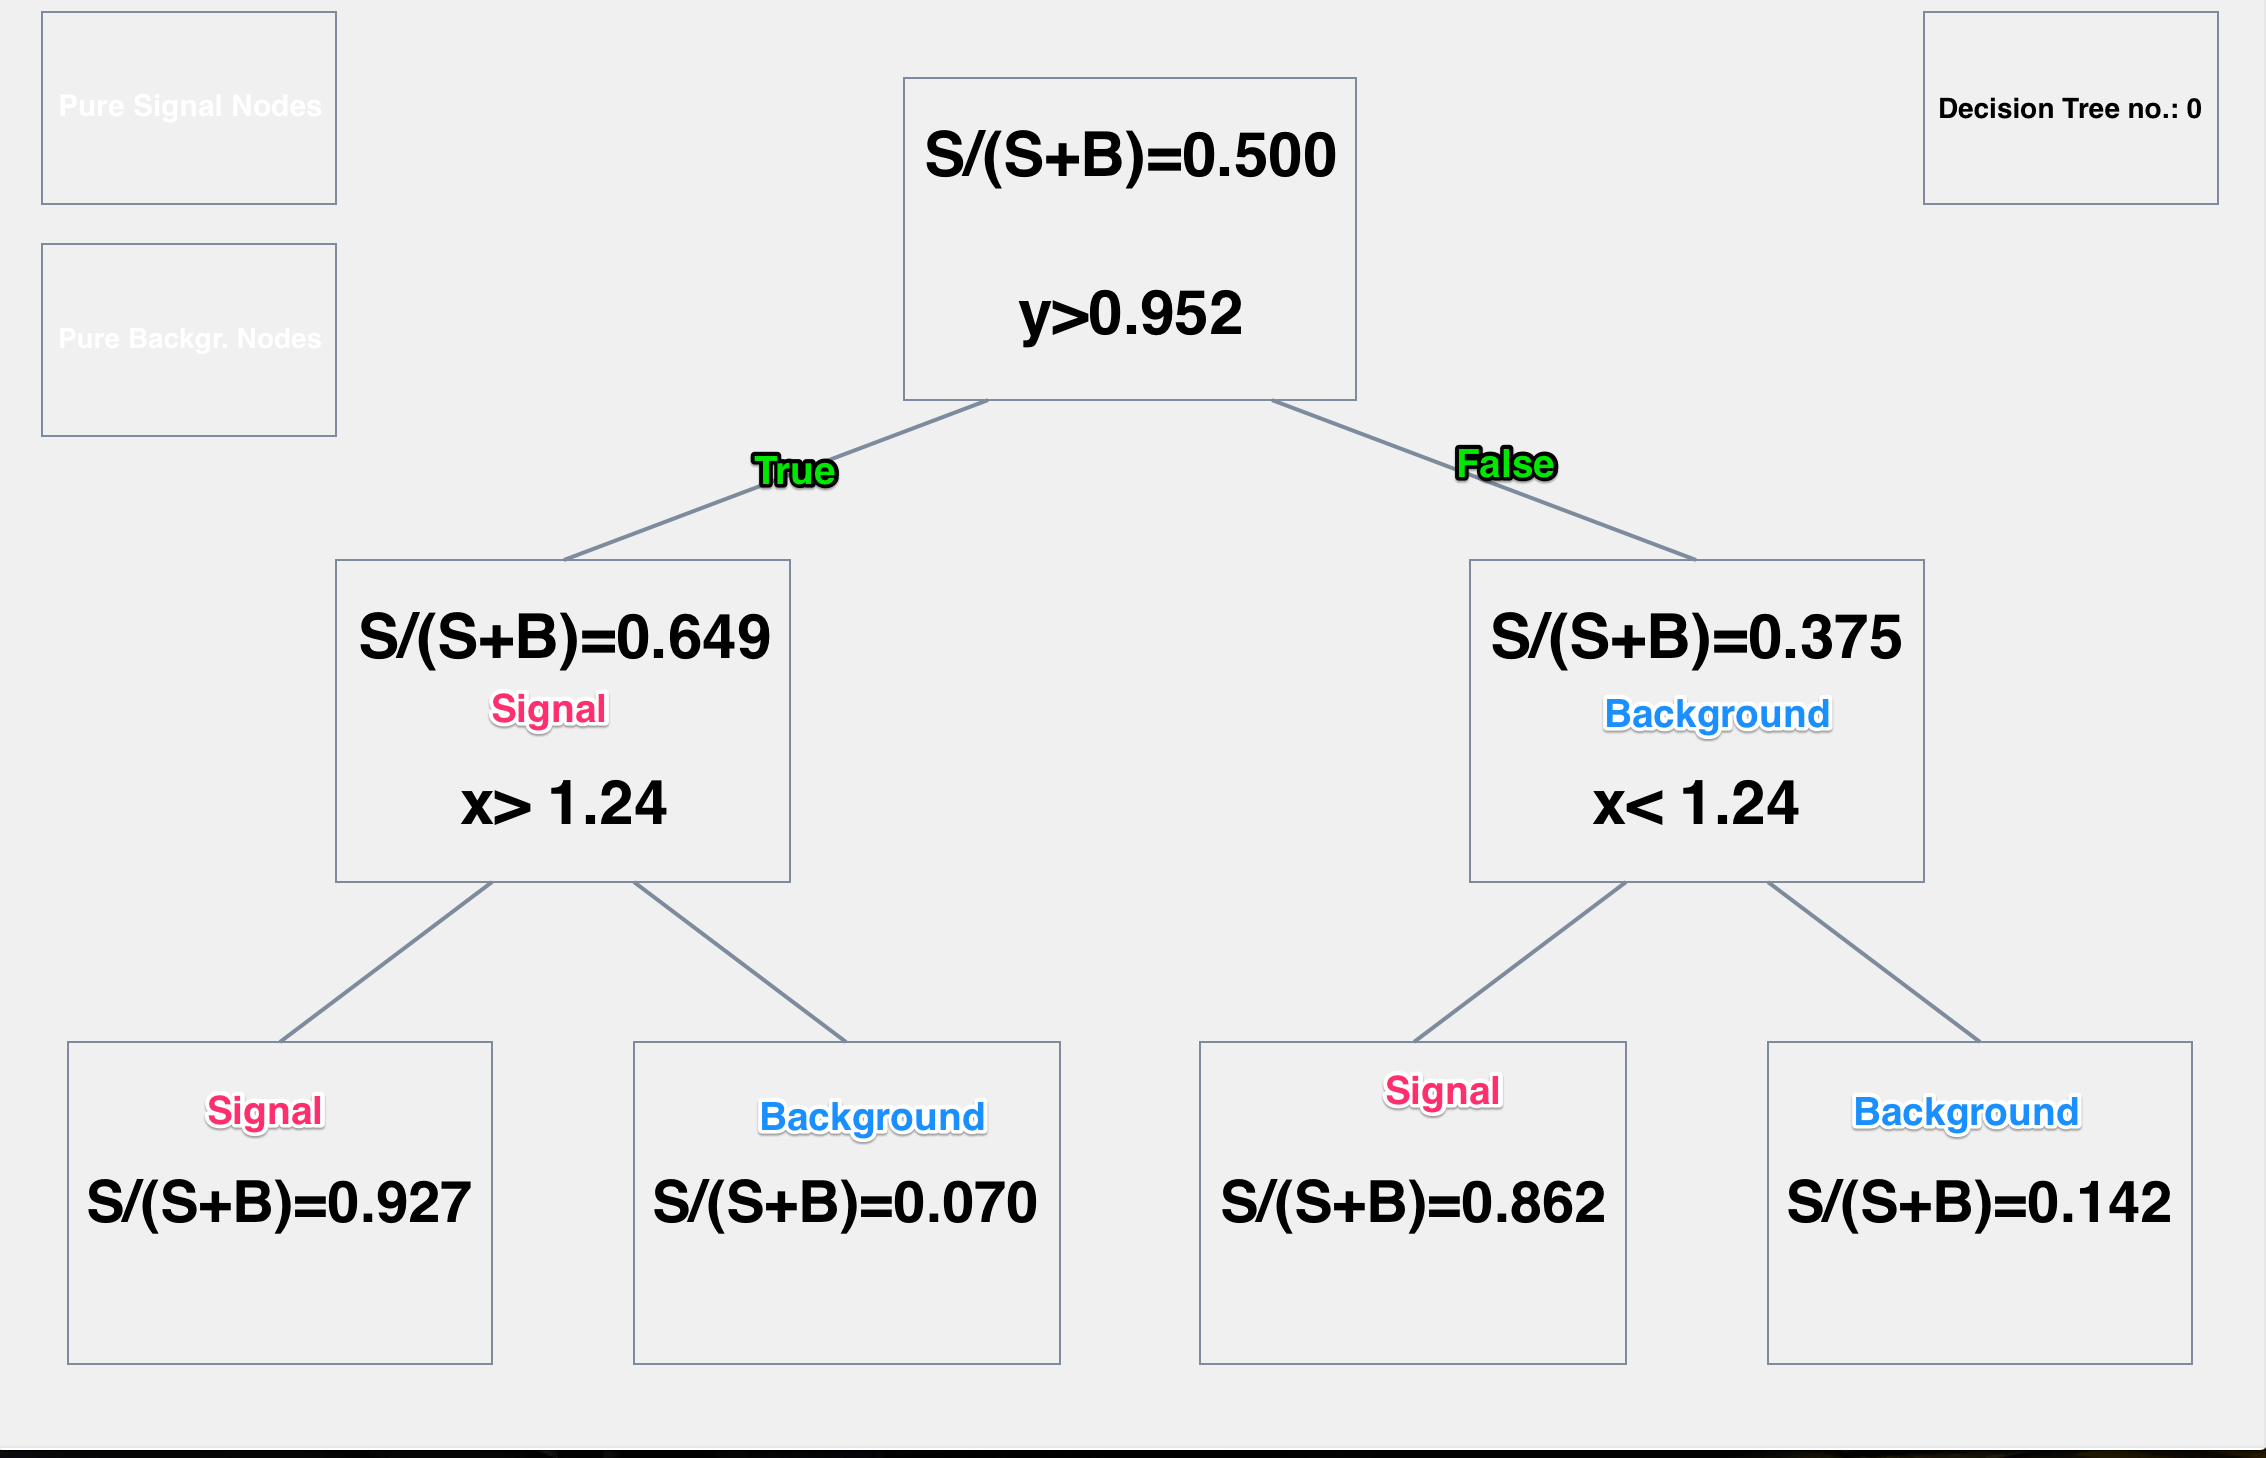
\includegraphics[width=\textwidth]{DT.png}
  \caption{A single decision tree that is classifying events as signal or background based on the artificial variables x and y}
  \label{fig:DT}
\end{figure}
\begin{figure}
  \centering
  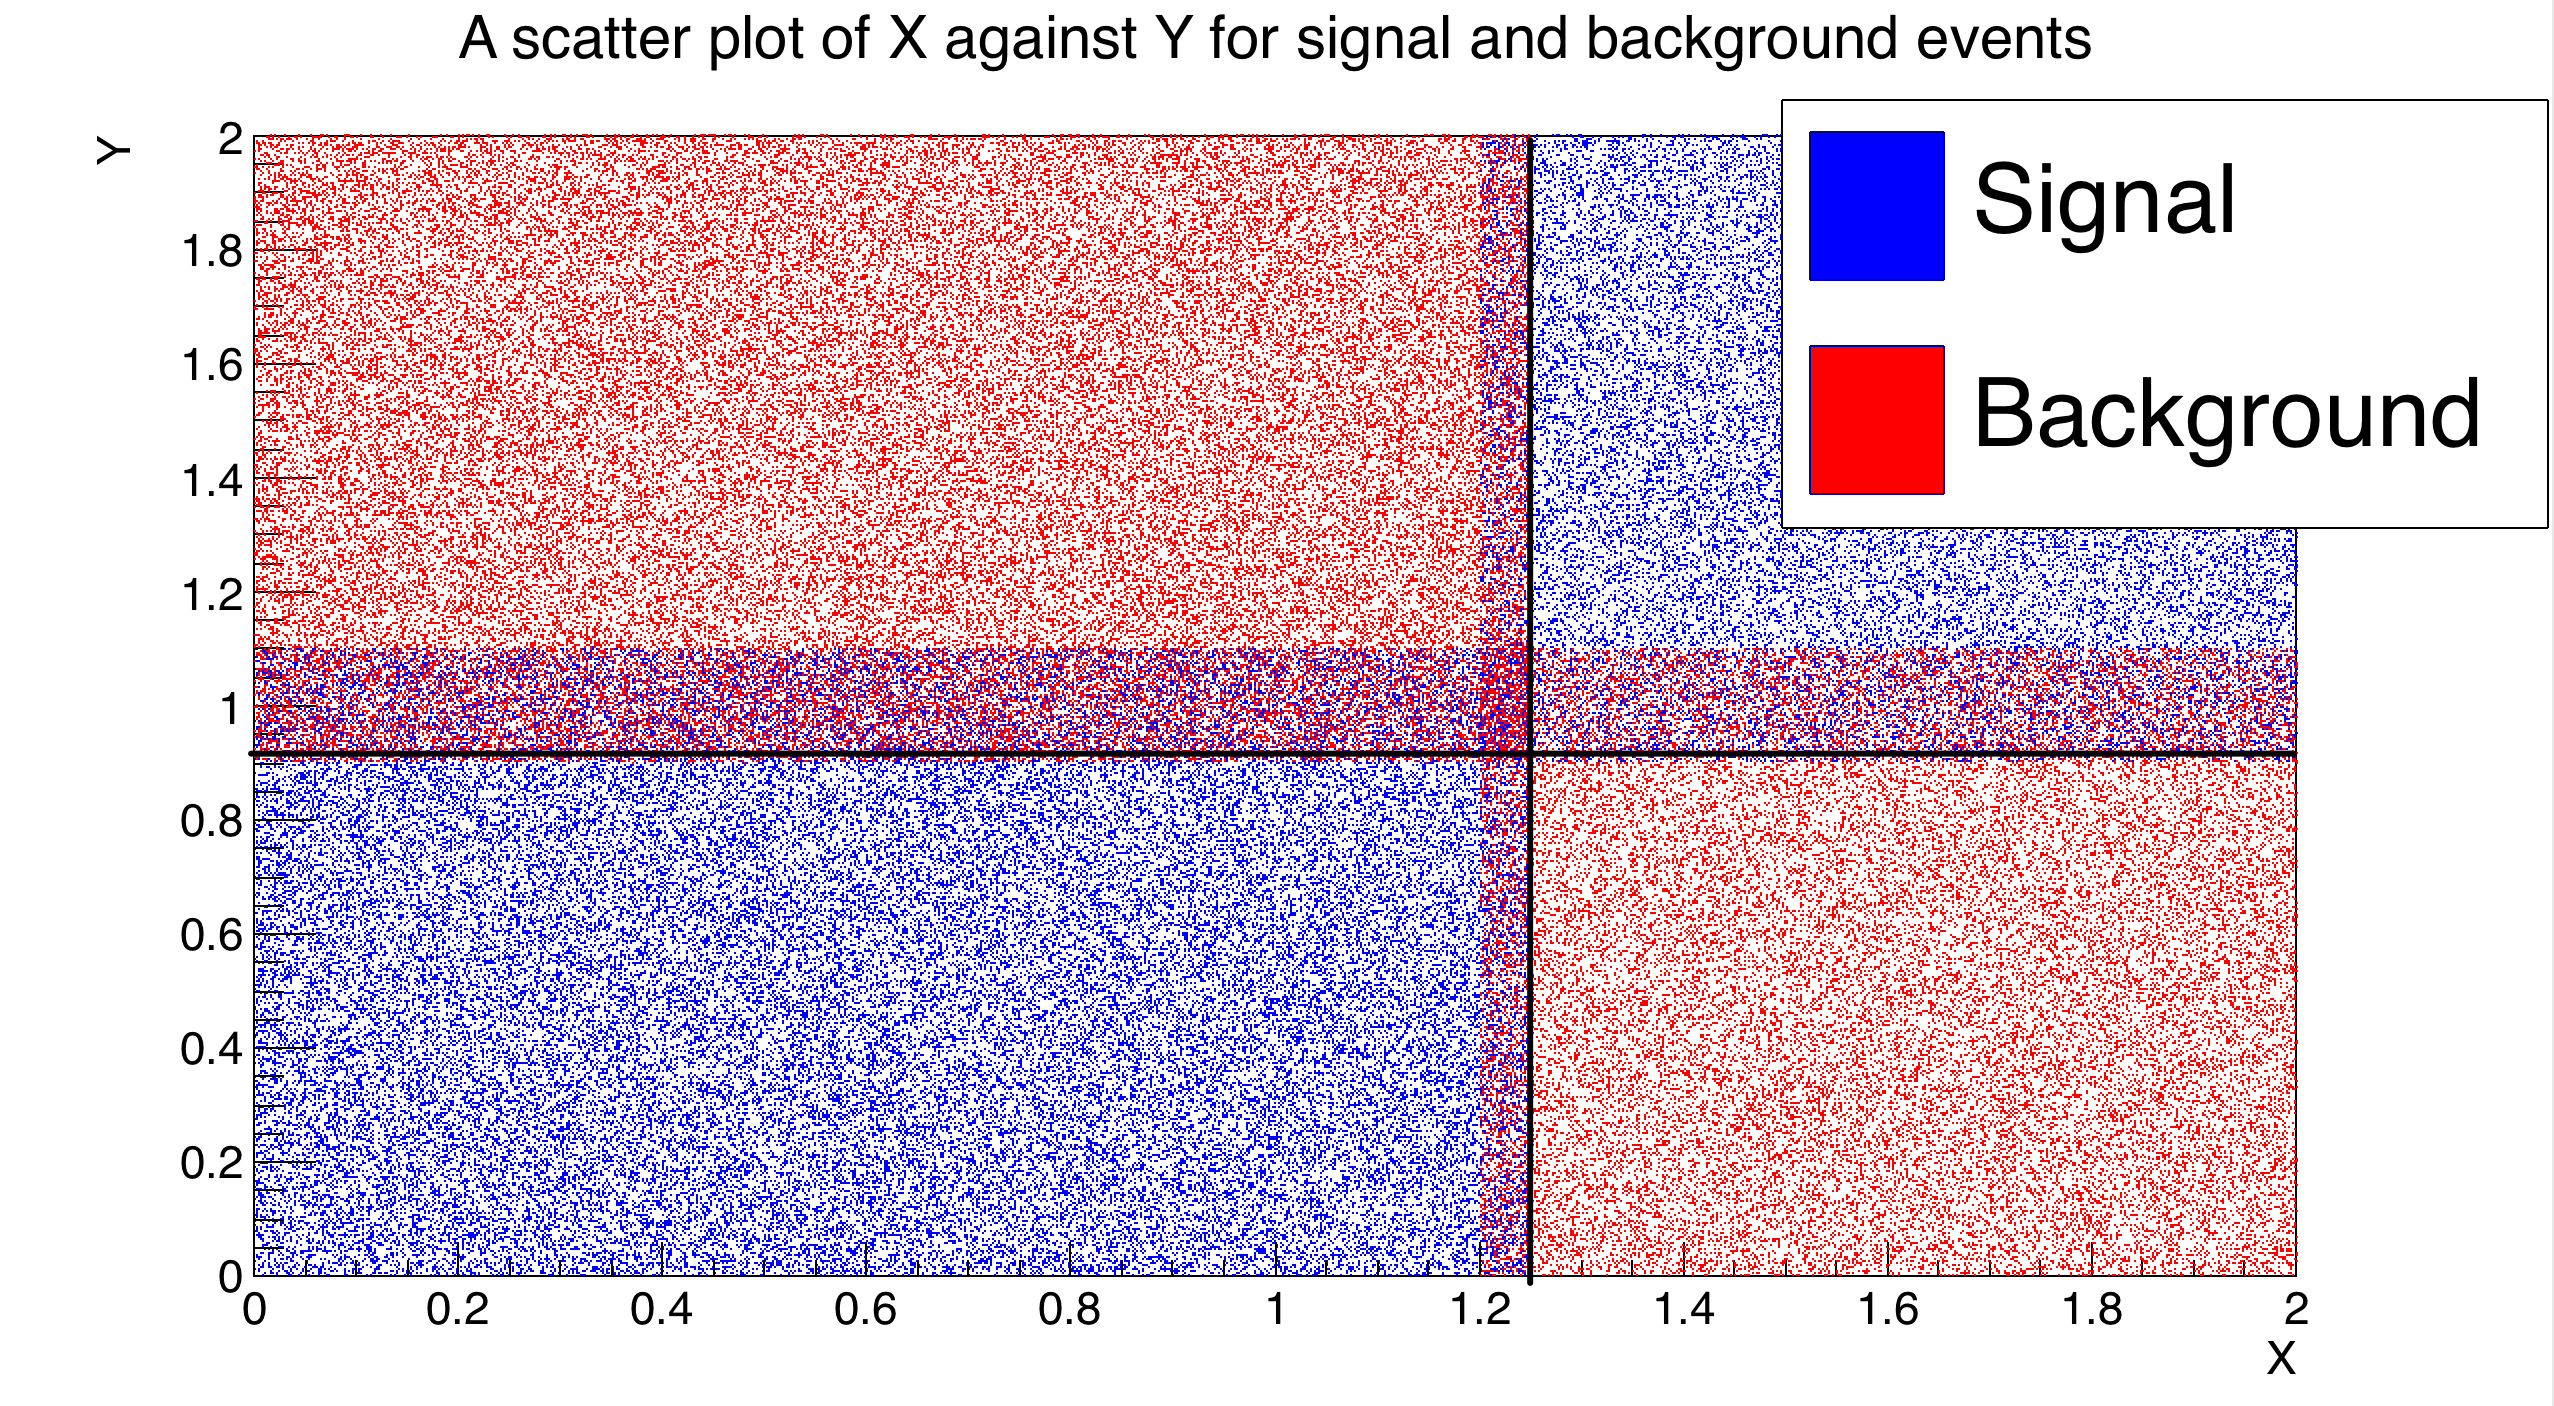
\includegraphics[width=\textwidth]{square.png}
  \caption{A scatter plot of $x$ against $y$ for the artificially generated events. The black lines show the cuts applied by the trained decision tree in Figure \ref{fig:DT}}
  \label{fig:square}
\end{figure}

It should be noted that the artificial variables provide better seperation than any found in real data but despite this there are still background events that are classified as signal events and vica versa. Also, it is not unusual for some analyses to use as many as 30 variables in a multi variate analysis which would make a single decision tre very complex.  The biggest reason why a single decision tree is not used, however, is because the training of a single tree is not stable; it is highly susceptible to statistical fluctuations.

\paragraph{Boosting}
These issues are solved by the boosting process, which involves training many decision trees (400-1200), scoring the effectiveness of the tree and returning a single value that is the weighted average of the response from all the trees.  In this analysis the TMVA package is used to train and apply BDTs which uses the Adaboost algorithm\cite{Hocker:2007ht}. 

After all the DTs are trained, the first step in the boosting process is to assign all events a weight $W=\frac{1}{m}$ where m is the number of events in the control sample.  To caluclate the score, $\alpha$, of each DT the fraction of events that are mis identified,E, is calcualted for every DT. This is another reason why control samples of known signal and background events are required for training.  A DT with a low value of E is chosen as the first DT to score and the value of $\alpha$ for that DT is calculated as,
\begin{equation}
  \alpha=\beta ln\big(\frac{1-E}{E}\big)
\end{equation}
where $\beta$ is a constant.  Next, the weights of events mis identified by the first DT are re assigned to be,
\begin{equation}
  W=W e^{\alpha}
\end{equation}
and all event weights are renomralised.  This lends more weight to mis idenitifed events. The same scoring process is then iteratively applied to every DT trained, but mis identified events are only re weighted until the total weight of all mis identified events reaches $50\%$. 

For a given event the final BDT value assigned is given by,

\begin{equation}
  V=\sum \limits_{i}^{N_{Trees}}\alpha_iV_i
\end{equation}

where $\alpha_i$ is the score assigned to the i'th decision tree and $V_i$ is the output of the $i_{th}$ decision tree which is -1 if the DT classifys the event as background and 1 if it is classified as signal.  This means the final value assigned to an event by the BDT is between -1 and 1 with 1 being more likely to be signal.  After the BDT is applied, there is a single BDT variable that can be cut on.

%TODO add adaboost reference.
\paragraph{Application for \Bd \to \Kstar \etaz}
A BDT was trained, and applied to candidates that passed the trigger and stripping selections to discriminate signal from combinatorial background.  Truth matched signal MC was used as a signal control sample and data with a refitted \Bd mass greater than 5500MeV was used as a background control sample to train the BDT.  This mass was chosen because it is far enough away from the real \Bd mass to definitely be background whilst still keeping a reasonable sample size.  Data from the lower mass sideband was not used for training as it is highly likely to contain partially reconstructed backgrounds rather than pure combinatorial background.  This would be a problem because BDTs are only effective for discriminating between two classes of events.

The variables used in the BDT are shown in Table \ref{tab:vars}.  The TMVA package ranks all input variables in order of importance based on the gini value and the number of times it is the variable in the top node of the tree.  These variables were chosen by adding all variables that could possibly discriminate signal from background and then iteratively removing the lowest ranked variables.  This was done until the lowest ranked variable still made a significant contribution to the signal and background seperation.  Care was also taken to ensure variables that are poorly modelled in MC were not used, as this could lead to false seperation.  Plots comparing a selection of these input variables in the signal and background control samples are shown in Figure \ref{fig:vars}.

\begin{table}[h]
  \label{tab:vars}
  \scriptsize
  \centering
  \begin{tabular}{|c|p{10cm}|}
    \hline
    Variable & Explanation \\ \hline
    B0 PT & Transverse momentum of \Bd candidate \\ \hline
    log(1-B0 DIRA OWNPV) & natural log of one minus the DIRA angle (see section \ref{sec:stripping}) \\ \hline
    B0 ENDVERTEX CHI2 & The $\chi^2$ probability of the \Bd endvertex from the least squares fit used to assign the daughters to the B0 endvertex \\ \hline
    log(B0 PVFit Chi2) & The natural logarithm of the $\chi^2$ of the fit used to refit the entire decaytree described in section \ref{sec:Decay Reconstruction} \\ \hline
    B0 eta & The pseudorapidity of the \Bd candidate \\ \hline
    B0 FD OWNPV & The flight distance of the \Bd between the primary vertex and decay vertex \\ \hline
    log(B0 TAU CHI2) & The $\chi^2$ probability of the \Bd lifetime. \\ \hline
    Kstar CosTheta & The cosine of the angle between the \Kstar candidates momentum in the \Bd rest frame and the \Bd momentum in the lab frame. \\ \hline
    Kstar eta & The pseudorapidity of the \Kstar \\ \hline
    piminus0 OWNPV CHI2 & The $\chi^2$ probability of the \pim belonging to the \etaz vertex \\ \hline
    pi0 CosTheta & The cosine of the angle between the \piz candidates momentum in the \etaz rest frame and the \etaz momentum in the lab frame.\\ \hline
    gamma PT and gamma0 PT & The transverse momentum of the photons from the \piz \\ \hline
    log B0RF KPlusKst costheta & The logarithm of the cosine of the angle between the \Kp and the \Kstar candidate in the rest frame of the \Bd. \\ \hline
    etaRF PiPlusPiMinus0 costheta & The cosine of the angle between the \pip and \pim from the \etaz in the rest frame of the \etaz. \\ \hline
    gamma0 CL and gamma CL & The probability that the photons from the \piz are actually photons.  This is assigned by the \lhcb calorimeter system. \\ \hline
    B0 Sum Track PT & The sum of the transverse momentum for all tracks in a candiate event (\pim,\Kp,\pim,\pip). \\ \hline
    B0 Sum PCHI2 & The sum of the $chi^2$ probabilities for each track belonging to the event. \\ \hline
    B0RF KPlusPiMinus costheta & The cosine of the angle between the \Kp and \pim in the rest frame of the \Bd \\ \hline

    %TODO check variable description
  \end{tabular}
  \caption{The variables used in the BDT, a diagram of the decay is shown in Figure \ref{fig:decaytree}}
\end{table}

\begin{figure}
  \centering
  \includegraphics[width=\textwidth]{vars.png}
  \caption{Plots of 6 of the input variables showing the seperation between signal and background they provide}
  \label{fig:vars}
\end{figure}

The overall ouptut of the trained BDT for the control samples is shown in Figure \ref{fig:BDTOut}.  Firstly, this plot shows that the BDT is able to provide good seperation between signal and background.  This plot also shows the overtraining check that TMVA performs.  Overtraining occurs when the BDT becomes too sensitive to statistical fluctuations in the input variable distributions.  In the case of overtraining, the BDT shows excellent seperation for the specific control samples used but worse seperation for the input variables in general.  TMVA checks for this by splitting the control samples in half before training, and only one half is used to train the BDT.  When the BDT is trained, it is applied to the remaining half of the control sampeles, and in the case of no overtraining the distirbution of the BDT response varaible should be the same for both halves of the control samples.  Figure \ref{fig:BDTOut} shows the BDT response distributions for both the training and test samples. These are considered to be consistent, there are no systematic disrepencies between the distributions.  The Kolomogrov-Smirnov test shown on the plot should be ignored, as internal \lhcb studies have shown this to be unreliable\cite{Grünberg:2019861}.  This trained BDT was then applied to all events that passed the stripping and trigger cuts.

\begin{figure}
  \centering
  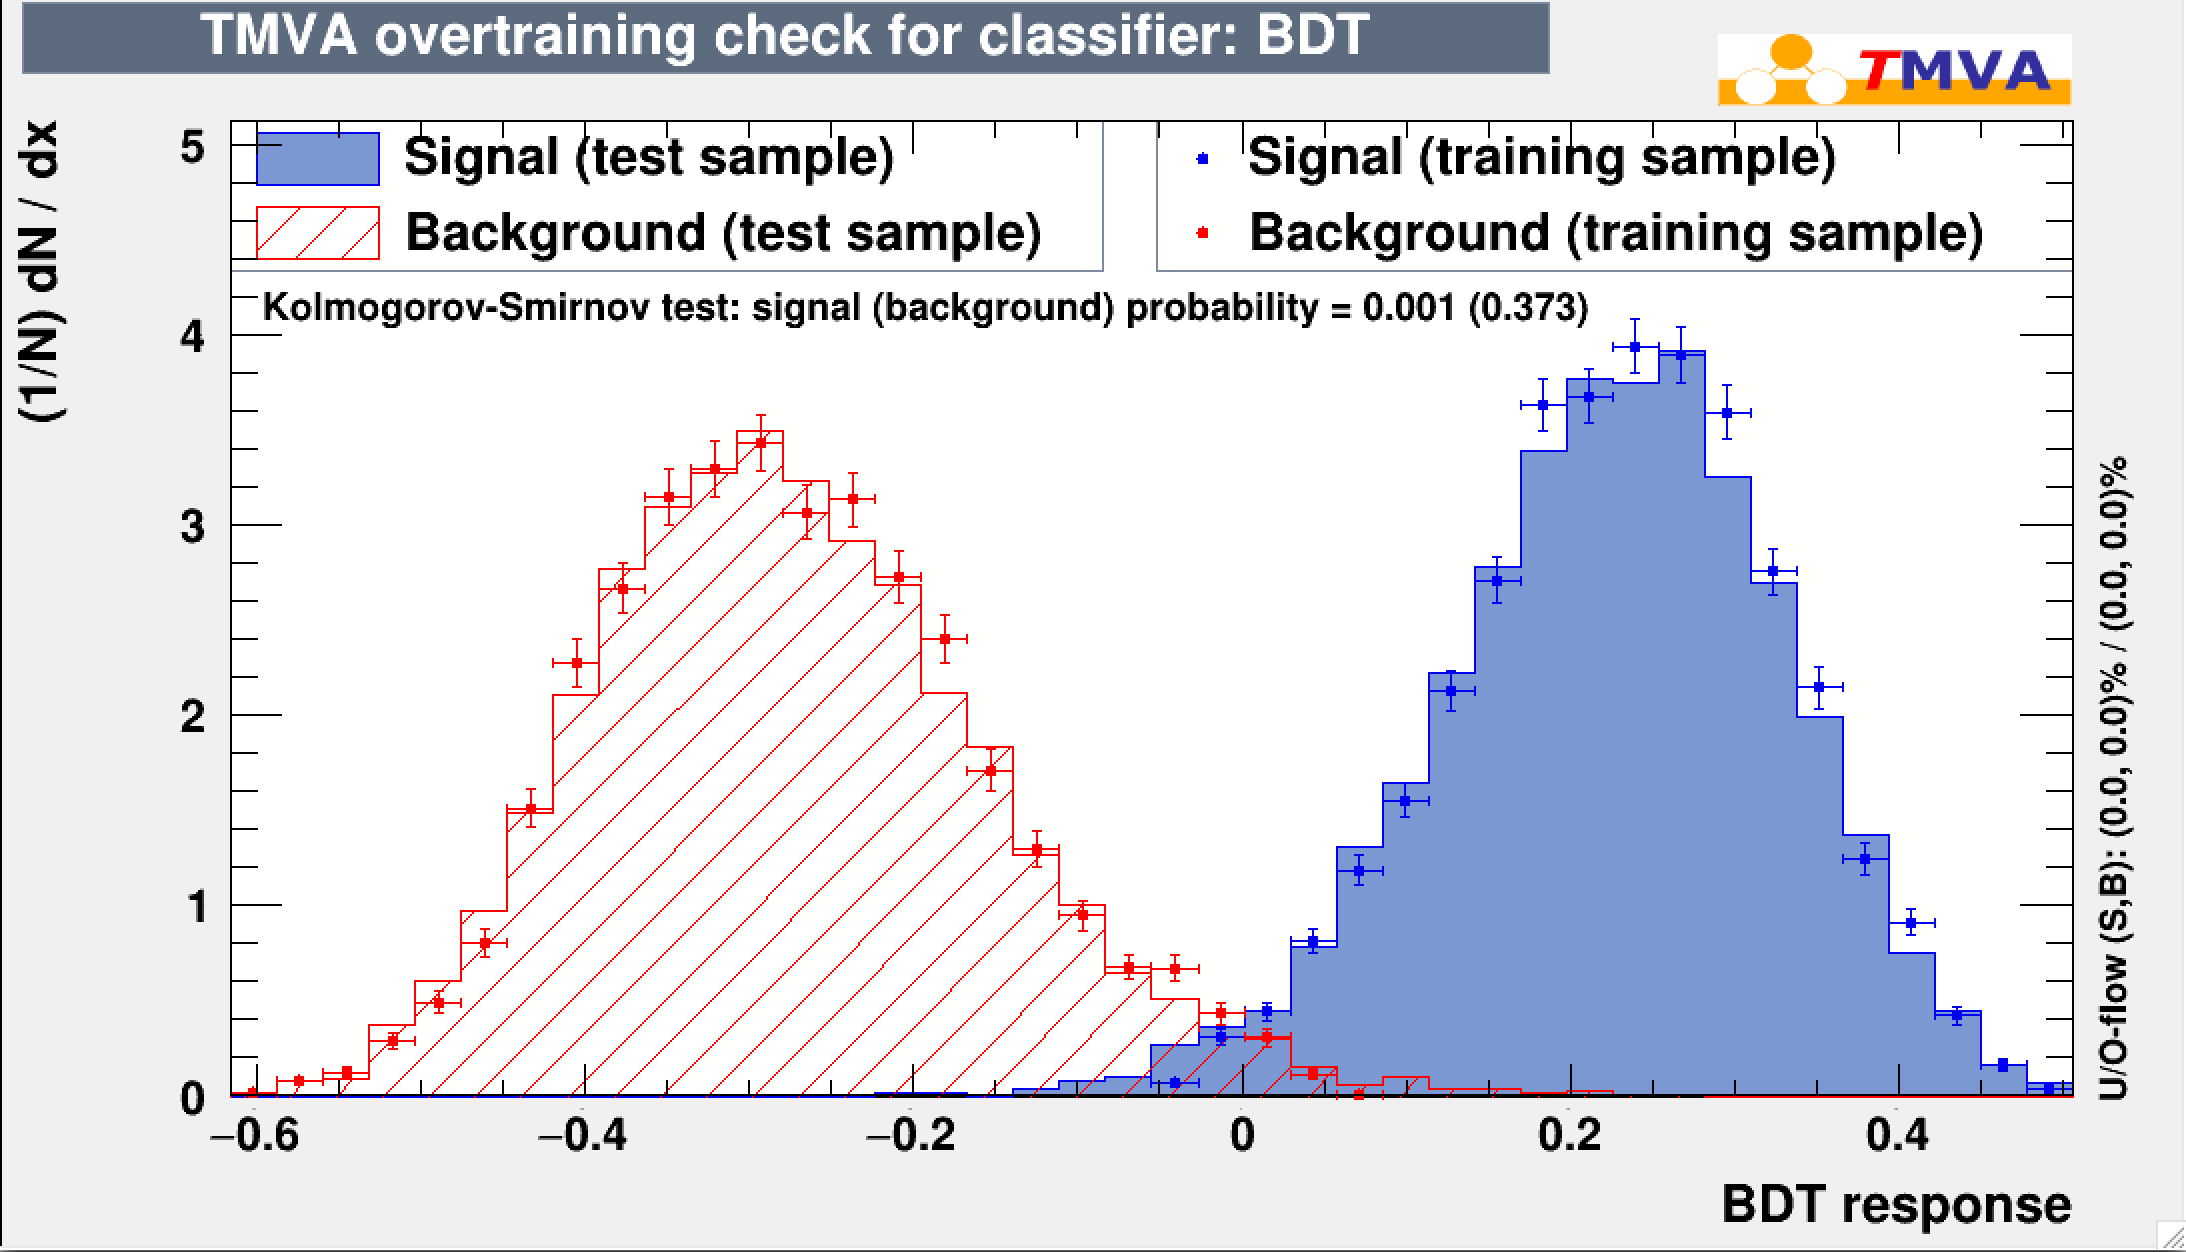
\includegraphics[width=\textwidth]{BDTOut.png}
  \caption{The output of the BDT as applied to the control samples.  This also shows the overtraining check}
  \label{fig:BDTOut}
\end{figure}
%TODO maybe do BDT double training thing

%optimisation of BDT Cut
\paragraph{Optimisation of BDT Cut}



%Decay Reconstruction
%Selection
%---Stripping
%---Trigger Selection
%---BDT
%---

\clearpage
